\documentclass[10pt,twocolumn,letterpaper]{article}
\usepackage{cvpr}
\usepackage{times}
\usepackage{graphicx}
\usepackage{amsmath}
\usepackage{amssymb}
\usepackage{xfrac}
\usepackage[pagebackref=true,breaklinks=true,colorlinks,bookmarks=false]{hyperref}

\def\GroupID{26} % <------- ENTER YOUR COMP6321 group number here

\begin{document}
\title{What {\em is} the Best Classifier?\\
       What {\em is} the Best Regressor?}
\author{Arjuman Mansuri\\(40076180) \and Manan Prajapati\\(40071095) \and Khyatibahen Chaudhary\\(40071098)}
\maketitle

\begin{abstract}
   This report investigates two questions.
   First, for a given selection of data sets, can we say what
   is the `best' classifier or the `best' regressor in terms
   of good predictions?
   How much does the answer depend on the particular selection of data sets?
   How much does the answer depend on our computational constraints?
   We investigate these questions using data sets from the UCI repository.
   Second, we compare the interpretability of a decision tree
   classifier to that of a convolutional neural network.
   We compare the decision tree visualization
   to `activation maximization', a technique to gain insight into
   the kinds of inputs that deep neural networks respond to.
   As a novelty component, we tried to understand the dropout technique used in neural networks for regularization and feature selection in general.
\end{abstract}



%------------------------------------------------------------------------
\section{Introduction}

The main aim of this report is to convey the tasks undertaken for identification
of the best classifier and regressor using supervised machine learning
techniques and interpretation of image classifiers trained on a dataset using
convolutional neural network and decision tree classifier. The project is based
on datasets from various sectors namely finance, health, industrial, crime,
education, social media, biology, product and multimedia from the UCI
repository. To accomplish the goal of this project, we trained and evaluated 8
classification methods across 10 classification datasets, 7 regression methods
across 10 regression datasets and 2 classification methods on an image
classification dataset.

At the start of the project, we performed an introductory analysis of each
diversified dataset to understand type and range of the features and output
labels involved. Since the datasets were in different formats (file types), we
loaded them using the corresponding libraries. Post data loading, we
preprocessed the data for identifying and replacing the missing values, encoded
alphabetical discrete values, performed feature selection and split dataset into
training and test set, if required and finally transformed it. After data
preprocessing, we trained the respective models using \textit{hyperparameter search}
technique and \textit{K-fold cross validation}, and evaluated the models based on their
predictive accuracies on the respective test sets to find the best regressor and
classifier.

The project also involved image classification by object recognition to be
performed on the classic CIFAR-10 dataset. The CIFAR-10 dataset consists of
60000 32x32 color images in 10 classes, with 6000 images per class. There are
50000 training images and 10000 test images. Since, the dataset contained images
in a binary format, we transformed them into a format good enough for
preprocessing. Subsequently, we preprocessed the data and prepared it for
training a Convolutional Neural Network (CNN). The same data was also used for
training a decision tree classifier. In the end, we compared the predictive
accuracies of both the models, to identify a better model.

As a part of the novelty component, we considered feature selection (described in the next section) and drop-out technique for neural network regularization (described in the conclusion section).

%------------------------------------------------------------------------
\section{Methodology \& Experimental Results}

% DELETE THIS TEXT
This section includes the details of methods used for preprocessing of raw
datasets and model selection by fine tuning of hyperparameters. In the
subsequent subsections the experimental results of the model accuracies are
compared to find the best model from the ones used.  The following content
would describe the common concepts and methodologies used irrespective of
the machine learning techniques used.

The first step while working with real world datasets is to identify noise
and inconsistency and preprocess the data by replacing missing values. It is
crucial to handle such ambiguities as they could lead to wrong prediction or
classification. Generally, missing values are represented by \textit{NaN,
empty string, ?, or --}. To identify missing values in our dataset we loaded
the dataset using pandas which helped to replace all the missing value
formats with \textit{NaN}. The number of missing values were counted per feature and
to identify features with missing values. We used different approaches for
replacing missing values as the approach is heavily dependent on the type of
the dataset. For numerical features, missing values were replaced by mean or
median of the that feature and categorical features were filled by most
frequent values encountered in that feature.

As the arrangement of features and output values was inconsistent across the datasets, we went through the dataset description, described on UCI repository and bifurcated our dataset into input and output sets.

Some of the given datasets have a large number of features which make it difficult to train a model on that dataset in a reasonable amount of time. Also, in such cases it is possible that some features have negligible contribution on prediction variable or output variable which can impact model’s performance. During the course of the project, two approaches were applied for feature selection depending on the nature and relation of the features with output variable. The first approach took into account the variance of the features and selected only those which pass a certain threshold of 0.9, i.e. feature having more than or equal to 90\% of the values same would be dropped. The other approach measured the correlation of each feature with the output values and drop the feature with negligible or zero correlation value.

Most of the datasets did not have a separate test dataset, so in order to test the model, we split the given dataset into training and testing set such that \sfrac{1}{3} of the dataset is considered as a testing set.

As machine learning models only understand numerical values, a dataset having alphabetical values needs to be encoded to numerical values. Such features were identified in all the datasets using pandas and encoded to numerical values using LabelEncoder of sklearn library.

Many of the datasets had features in highly different ranges of magnitudes which would deceive machine learning algorithms to predict a wrong value as it considers the Eucledian distance between two data points. This would result in the high magnitude features to dominate and bias the predictions towards them. To prevent this and ensure that the features with small magnitudes contribute equally, it is necessary to scale the feature values. While scaling the features, it is important to only fit the training data and not the test data to the scalar and then transform both of them.

Most of the machine learning models need appropriate hyperparameter settings in order to get a good accuracy on predictions. Different methods have different type and number of hyperparameters. The specifics of hyperparameter tuning depending on the type of experiment, have been discussed in the further sub-sections.

We tried a range of different hyper-parameter settings and finally settled with the one that resulted in the maximum accuracy. We used these selected hyperparameters to search over and find the best combination of them using Grid Search and Randomized Search as required. Randomized Search approach samples parameters from the provided choices via a random uniform distribution. In contrast to this, Grid Search tuning algorithm tries each and every combination of the hyper-parameter values. We observed that unless the search space of the hyper-parameters is small and can be easily enumerated, Randomized Search proves to be more efficient and less time-consuming.

Generally, datasets have data with varying variance for each of the features. So, according to the traditional convention, if the data is split just once then, the model captures the characteristics of only the training data and is tested only once by the test data. This does not prove to be efficient in terms of accuracy as not all the variance in the data is captured. K-fold cross validation divides the data into k folds and trains and validates the model for k iterations leading to a better trained model capturing all the variations in the data. For our project, we used 3-fold cross validation as it takes a moderate amount of time to train a model along with giving a good accuracy.

For instance, if a model had 6 different combinations of parameters and 3-fold cross validation, 18 cross-validated randomized grid searches would be performed.

The combination of Randomized Search and cross validation would yield the best estimator from all trained by them for a particular dataset. From our experiment, we observed that for Yeast dataset, Randomized Search took 30s and exhaustive Grid Search took 60s, proving that Randomized Search is faster along with exploring different regions of the optimization surface.


\subsection{Classification Experiments}

% DELETE THIS TEXT
The classification experiments were done on the following datasets:
Diabetic Retinopathy, Default of credit card clients, Breast Cancer Wisconsin, Statlog (Australian Credit approval), Statlog (German credit data), Steel Plates Fault, Adult, Yeast, Thoracic Surgery Data, Seismic-Bumps.
These datasets were to be classified using the following models:
k-nearest neighbour classification, Support vector classification, Decision tree classification, Random forest classification, AdaBoost classification, Logistic regression (for classification), Gaussian naive Bayes classification, Neural network classification.
While training these models, we used a few hyper-parameters corresponding to the model which are as follows: 
\\*\textit{KNeighborsClassifier: 'n\_neighbors', 'metric',
\\*SVC: 'kernel', 'C', 'gamma',
\\*'DecisionTreeClassifier': 'criterion', 'max\_depth'
\\*'RandomForestClassifier': 'n\_estimators'
 \\*'AdaBoostClassifier': 'n\_estimators', 'learning\_rate',
  \\*'LogisticRegression': 'max\_iter','C', 'solver'
    \\*'MLPClassifier': 'hidden\_layer\_sizes', 'activation'}
    
Hyperparameter settings have a high dependence on the size of the dataset. To provide an example of such hyper-parmeters, we will consider Logistic Regression as the model at hand. For the ‘solver’ hyper-parameter, the value ‘liblinear’ would work well with smaller datasets, whereas ‘sag’ and ‘saga’ converged faster for the larger ones. So, for the datasets with a few thousand number of rows, most of the Logistic Regression models used ‘liblinear’, except for the larger datasets like the Adult dataset consisting of 32,561 records.

Machine learning model evaluation is highly dependent on the distribution of the classes in the dataset. So, after checking the class distributions in the data information files of the datasets, we decided different performance metrics for each dataset. If the classes were equally distributed then, we would have used accuracy which would report the number of correct predictions made over all the predictions. But since most of the datasets had class imbalance, we utilized f1 score which represents both precision (the proportion of positive identifications that were actually correct) and recall (the proportion of actual positives identified correctly). Figure \ref{first_figure} shows class imbalance in the Steel Plates Fault dataset.

In order to compare the performance of different models on a single dataset, we generated an accuracy vs best estimator model bar graph as depicted in Figure \ref{second_figure}.
Here, we have included a graph of the same Steel Plates Fault dataset.

\subsection{Regression Experiments}

% DELETE THIS TEXT
The regression experiments were done on the following datasets:
Wine Quality, Communities and Crime, QSAR aquatic toxicity, Parkinson Speech, Facebook metrics, Bike Sharing, Student Performance, Concrete Compressive Strength, SGEMM GPU kernel performance, Merck Molecular Activity Challenge.
These datasets were to be classified using the following models:
Support vector regression, Decision tree regression, Random forest regression, AdaBoost regression, Gaussian process regression, Linear regression, Neural network regression.
While training these models, we used a few hyper-parameters corresponding to the model which are as follows: 
   \\*\textit{ SVR: 'C', 'gamma',
   \\* DecisionTreeRegressor:     \\*'max\_depth','min\_samples\_leaf','min\_samples\_split',
    \\*RandomForestRegressor: 'max\_depth','n\_estimators',
    \\*AdaBoostRegressor: 'n\_estimators','learning\_rate',
    \\*GaussianProcessRegressor: 'normalize\_y',
    \\*MLPRegressor:\\'hidden\_layer\_sizes','activation', 'max\_iter',}
    
Hyperparameter settings have a high dependence on the number of inputs and outputs of the dataset. To provide an example of such hyperparmeters, we will consider \textit{MLPRegressor (Multilayer Perceptron Regressor)} as the model at hand. The ‘hidden\_layer\_size’ hyper-parameter includes the number of hidden units in each layer and the number of layers in the model. There are various ways of determining the size of the hidden layer depending on the size of the input like \sfrac{2}{3} of the input or mean of the input and output. But, that led to very large numbers which were infeasible for us to train the model on. So, we selected a relatively small number of layers depending on the size of the input.

For the regression models, we have considered three kinds of evaluation metrics namely \textit{Mean Squared Error (MSE), Root Mean Squared Error (RMSE) and R Squared Score (R2)}. MSE calculates the distance between the actual and the predicted value and sums it for all the inputs. Among some limitations of MSE, the major one is that it might deceive us in believing a good model as a bad one if one of the inputs predicted a value very far from the actual value and vice-versa. RMSE is the root of MSE to make scale of the errors same as the scale of the targets. R2 is simply the amount of variance captured by the model. During the experiment, we calculated both kinds of errors, RMSE and R2 for all the datasets and considered the one that could explain the variance in the data appropriately. If RMSE for a particular dataset was not interpretable, we calculated R2 for that dataset.
In order to compare the performance of different models on a single dataset, we generated a graph similar to the one for classification experiment.


\subsection{Interpretability Experiments}

% DELETE THIS TEXT
This part of the experiment included training a \textit{Convolutional Neural Network (CNN)} on CIFAR 10 dataset. Data loading for this dataset was a bit different from the other datasets as the data was in bytes format. Also, the CNN model was built using \textit{pytorch}, so the data was encapsulated in tensors. The images were in RGB channels with dimension of 32 x 32 pixels. 
After pre-processing was done, we built a model including the following specifications:
\begin{enumerate}
\item Convolution with 5 different filters in size of (4x4) with \textit{ReLU} activation function:
\\*Given that the input image is in 3 channels, the in\_channels were 3. Here, we applied 5 different feature detectors and hence the number of out\_channels is 5. The filter size of each of the feature detectors at this layer was 4. Hence, this reduced the size of the output image to 29 x 29 feature maps. Since, the number of out\_channels was 5, 5 feature maps were created at the end of this convolutional transformation. The ReLU activation function would help to threshold all the incoming features to 0 or greater.
\item Convolution with 6 different filters in size of (6x6) with ReLU activation function:
\\*The number of out\_channels would serve as the number of in\_channels in this layer. In this case it would be 5. At this stage, the filter size of each of the feature detectors was 6 and 6 such detectors were used. Hence, this reduced the size of the output image to 24 x 24 feature maps. Since, the number of out\_channels was 6, 6 feature maps were created at the end of this convolutional transformation. ReLU activation function would perform the similar operation as in the previous layer.
\item Max Pooling by 2
\\*While performing the max pooling operation, kernel with kernel\_size 2 and a stride of 2 is selected. This would lead to a reduction in the dimensions of the output image by half i.e.12. This operation helps to drastically reduce the dimensions of the output feature maps along with preserving the most important features.
\item Flattening the 6-D output of the last convolving operation
\\*This operation would flatten the 6 x 12 x 12 max pooled output to 1 dimension so as to feed it to a fully connected neural network.
\item Fully Connected Layer with 864 input units and 10 output units
\\*This layer would serve as a neural network with 864 inputs and 10 output units corresponding to the 10 classes of the dataset images.
\end{enumerate}
A figure \ref{fourth_figure} explaining the architecture of the CNN network has been attached at the end of the report.

After considerable attempts, we settled on a batch\_size of 100, learning rate of 0.006 and momentum of 0.9. To perform back-propogation and optimization, \textit{CrossEntropyLoss} and \textit{Stochastic Gradient Descent} was used respectively. We tried a wide range of epochs and found out that this model gave the lowest loss at \textbf{epoch 13}.

After the model was trained successfully, we tried to visualize the activations caused by each convolutional layer. We loaded each layer from the model and fed data generated by the previous layer to it. This resulted in activations getting generated at each layer and we visualized them by plotting them. Activations for airplane, automobile, dog and cat generated by the plotting function are shown in figure \ref{seventh_figure}, \ref{fifth_figure} and \ref{sixth_figure}.
The same dataset was used to train a Decision Tree Classifier using a Grid Search Cross-Validation model to get the best estimator, whose accuracy was measured using the accuracy\_score metric.
Since the decision tree classifier had a large depth, we were able to visualize the model only upto a depth of 2 layers. In contrast to this, the results of activation maximization were highly interpretable as their visual representations depicted the objects (airplane, automobile, cat and dog) that needed to be classified.According to the accuracy scores of both the models, it is evident that CNN is better at classifying CIFAR 10 dataset’s images.





%------------------------------------------------------------------------
\section{Conclusions}

In terms of good predictions from our observations, it is difficult to have a single best classifier, as Random Forest Classifier, Support Vector Machine (SVM) and Multi-Layer Perceptron models were very close. But, in general, for all the datasets, \textbf{Random Forest Classifier} proved to give the best accuracies. While in the case of regression, it was not as difficult to decide the best model.  \textbf{Random Forest Regressor} proved to be the best regressor among all the models in terms of good predictions.
For classification, the performance of SVM is largely dependent on the size of the dataset. If the dataset grows beyond a certain size, the performance of SVM deteriorates while the same remains unchanged for Random Forests. For the classification and regression experiments, the conclusion is based on the observation that, to build multiple decision trees, random forest classifier and regressor randomly select rows and features and then averages the result, hence capturing all the variance in provided datasets. Hence, it proves to be excellent on unexpected validation datasets.
For both experiments, the computational constraint does not prove to be a blocker as random forest runtimes are quite fast.

While doing research for the novelty component, we realized that in some of the classification datasets, we observed that in spite of the training accuracies being excellent for the MLPClassifier, the test accuracies were quite low. We investigated to know later that it was caused due to overfitting of the training data with the model. This motivated us to introduce dropout technique in those neural networks. This not only helped us to increase the test accuracy but also increased the training speed as some of the neurons contributing to overfitting were removed by drop-out technique.

\begin{thebibliography}{10}

\bibitem{ref1}
TowardsDataScience\newblock Handle missing value
\newblock {https://towardsdatascience.com/the-tale-of-missing-values-in-python-c96beb0e8a9d},.
\newblock {https://towardsdatascience.com/6-different-ways-to-compensate-for-missing-values-data-imputation-with-examples-6022d9ca0779},.

\bibitem{ref3}
AppliedMachineLearning\newblock Cifar-10
\newblock {https://www.google.com/amp/s/appliedmachinelearning.}\\{blog/2018/03/24/achieving-90-accuracy-in-object-recognition-task-on-cifar-10-dataset-with-keras-convolutional-neural-networks/amp/},.

\bibitem{ref4}
TowardsDataScience\newblock Efficient Neural Architecture
\newblock {https://towardsdatascience.com/a-guide-to-an-efficient-way-to-build-neural-network-architectures-part-i-hyper-parameter-8129009f131b},.

\bibitem{ref5}
Adeshpande-Github\newblock Understand CNN
\newblock {https://adeshpande3.github.io/adeshpande3.github.io/A-Beginner\%27s-Guide-To-Understanding-Convolutional-Neural-Networks/
},.

\end{thebibliography}

\appendix
\begin{figure*}
   \begin{center}
   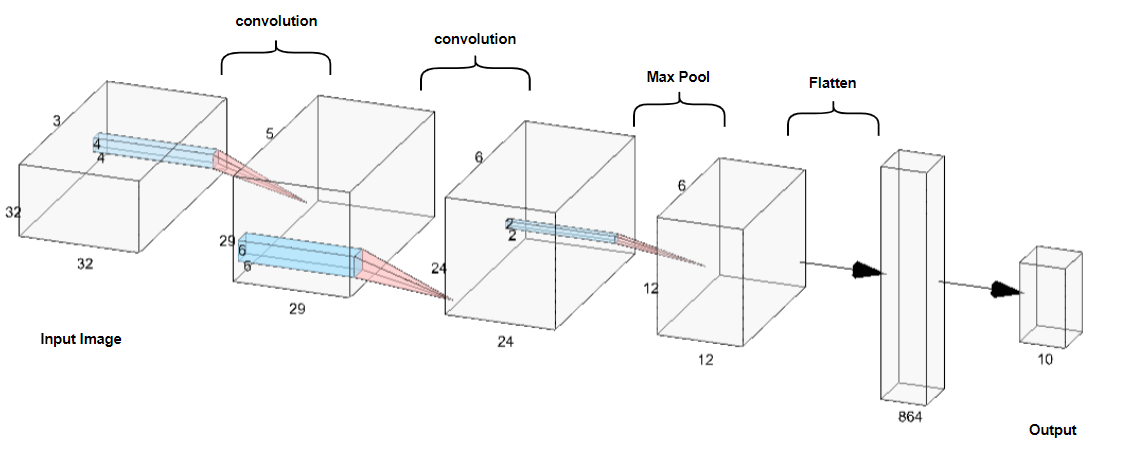
\includegraphics[width=\linewidth]{CNN_CIFAR10.PNG}
   
   \end{center}
     \caption{Architecture of CIFAR-10 CNN\label{fourth_figure}} 
\end{figure*}
% DELETE THIS FIGURE

\begin{figure}
\begin{tabular}{cc}
  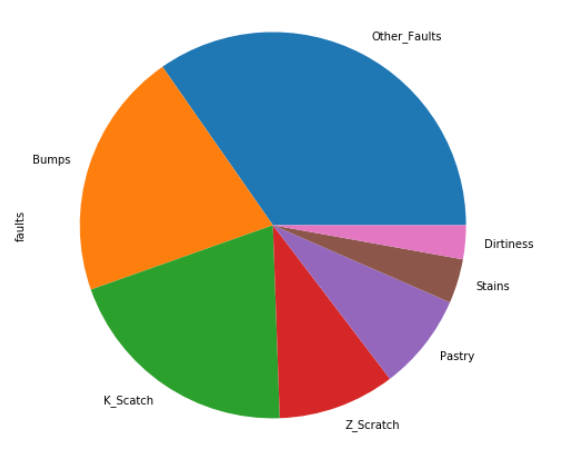
\includegraphics[width=80mm]{plot_1.PNG} &   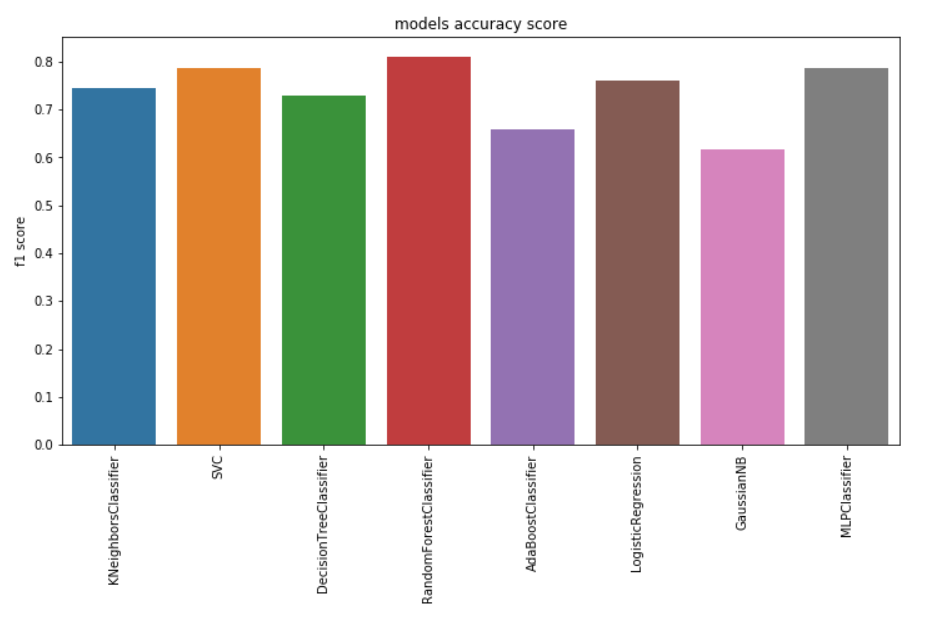
\includegraphics[width=80mm]{plot_2.PNG} \\
\caption{Pie-Chart of class labels (Steel Plates Faults)\label{first_figure}} & \caption{Plot of Model Accuracy\label{second_figure}}\\[6pt]
 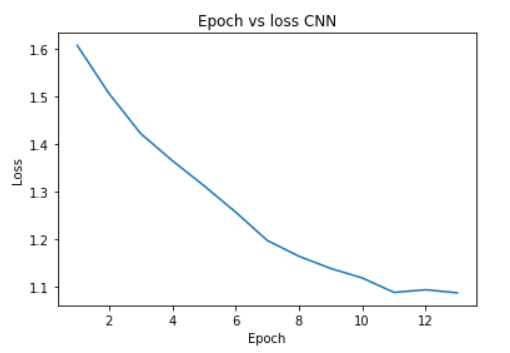
\includegraphics[width=80mm]{EpochVsLossCNN.PNG} &   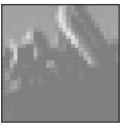
\includegraphics[width=40mm]{airplane.PNG}\\
\caption{Plot of Model Accuracy\label{third_figure}} & \caption{Airplane Activation\label{seventh_figure}}\\[6pt]
\end{tabular}
  
   \begin{center}
      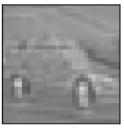
\includegraphics[width=0.3\linewidth]{car.PNG}
      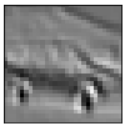
\includegraphics[width=0.3\linewidth]{car2.PNG}
   \end{center}
      \caption{Car Activation\label{fifth_figure}}
    \begin{center}
      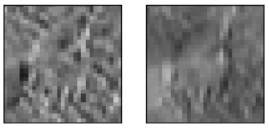
\includegraphics[width=0.6\linewidth]{cat_dog.PNG}
    \end{center}
      \caption{Dog and Cat Activation\label{sixth_figure}}
    
\end{figure}





\end{document}
